% =============================================================================
% sections/design/rover/rover_overview.tex  -  Rover Overview
% Teams: PM (best guess - unconfirmed) / Status: draft
%
% Content required:
%   - Rover's scheme with sizes
%   - Rover's photo #1
%   - Rover's photo #2
% Evidence-first rule (ai_context/DECISIONS.md): lead with the
% scheme/photos, keep prose to what the figures cannot say.
%
% Images below are placeholders (figures/rover_scheme.png,
% figures/rover_photo_1.png, figures/rover_photo_2.png) - swap them for the
% real scheme/photos by overwriting the same files, no need to touch the
% LaTeX layout.
% =============================================================================

The chassis is the rover structural platform integrating all major
subsystems in a four-wheel rocker-bogie layout built from aluminium
profiles, shown in \autoref{fig:rover_scheme}. An external differential
link couples the rocker arms and balances left-right terrain loads for
stability. Preliminary dimensions are approximately
\qtyproduct{1.2 x 0.8 x 0.7}{\meter} (L $\times$ W $\times$ H), subject to
refinement during detailed design. All four wheels are driven and steered,
each with a full \ang{360} steering range. The assembled rover is pictured
in \autoref{fig:rover_photos}.

\begin{figure}[!htbp]
    \centering
    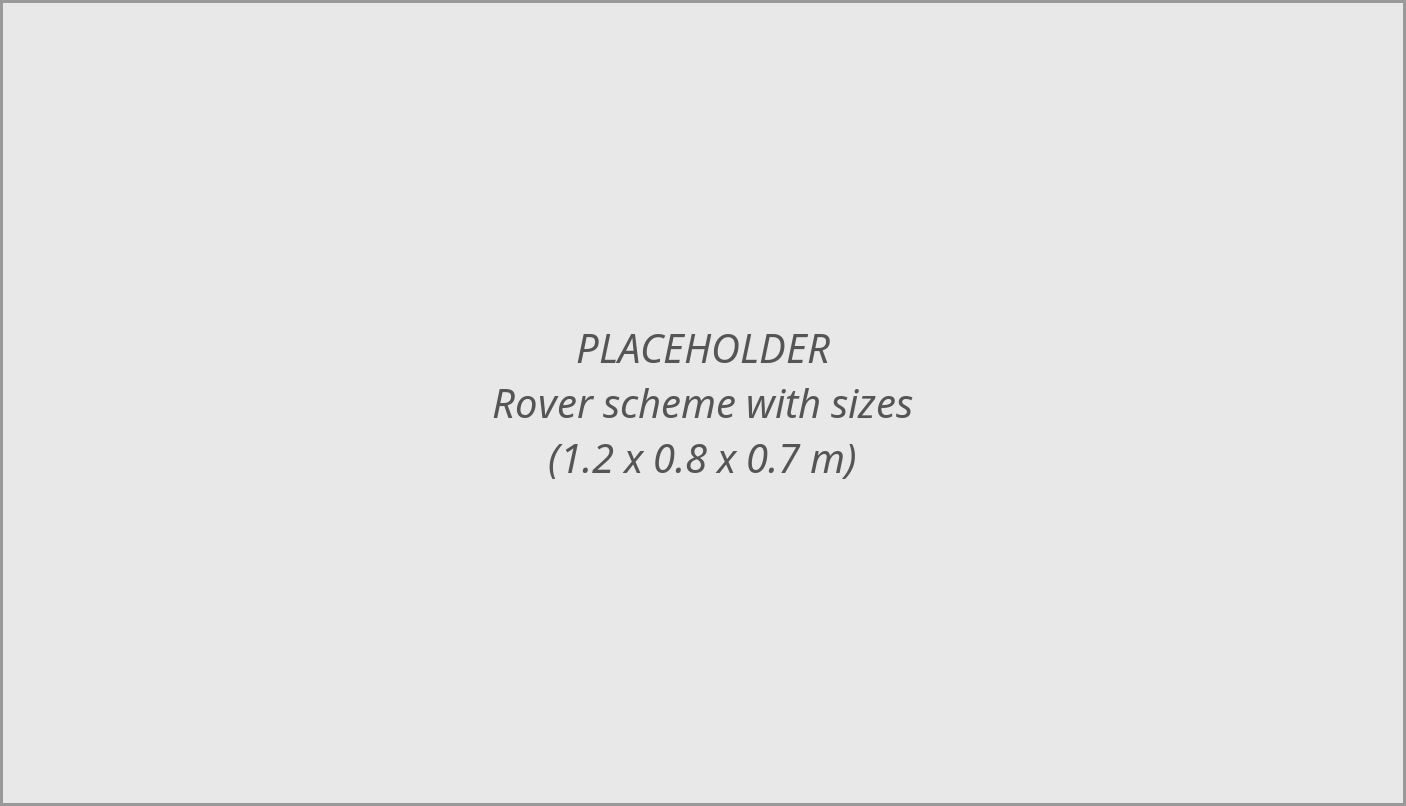
\includegraphics[width=0.8\linewidth]{figures/rover_scheme}
    \caption{Indomitus rover -- structural scheme with dimensions}
    \label{fig:rover_scheme}
\end{figure}

\begin{figure}[!htbp]
    \centering
    \setlength{\fboxsep}{0pt}

    \begin{minipage}[c]{0.49\textwidth}
        \centering
        
\includegraphics[height=3.5cm, keepaspectratio]{figures/rover_photo_1}
    \end{minipage}
    \hfill
    \begin{minipage}[c]{0.49\textwidth}
        \centering
        
\includegraphics[height=3.5cm, keepaspectratio]{figures/rover_photo_2}
    \end{minipage}

    \caption{Indomitus rover -- assembled system, photo \#1 (left) and photo \#2 (right)}
    \label{fig:rover_photos}
\end{figure}
